%%%%%%%%%%%%%%%%%%%%%%%%%%%%%%%%%%%%%%%%%
% Engineering Calculation Paper
% LaTeX Template
% Version 1.0 (20/1/13)
%
% This template has been downloaded from:
% http://www.LaTeXTemplates.com
%
% Original author:
% Dmitry Volynkin (dim_voly@yahoo.com.au)
%
% Revisions:
% TEC 5-29-2014 Updated for MATH 605 and OENG 644
%
% License:
% CC BY-NC-SA 3.0 (http://creativecommons.org/licenses/by-nc-sa/3.0/)
%
%%%%%%%%%%%%%%%%%%%%%%%%%%%%%%%%%%%%%%%%%

%----------------------------------------------------------------------------------------
%	PACKAGES AND OTHER DOCUMENT CONFIGURATIONS
%----------------------------------------------------------------------------------------

\input{packages_DocConfigs}

%----------------------------------------------------------------------------------------
%	HEADER INFORMATION
%----------------------------------------------------------------------------------------

\fancyhead[r]{\begin{tabular}{L{3cm} R{3cm} | L{3cm} R{5cm}} % The header is a table with 4 columns
\textbf{Author}   & Tim Coon & \textbf{Page}         & \thepage/\pageref{LastPage} \\
\textbf{Date}      & 11/22/14 & \textbf{Course}      & MECH 622 \\
\textbf{Description} & Qual Q\#2     & \textbf{Reference} & Cobb \& Dillsaver \\
\end{tabular}}

%----------------------------------------------------------------------------------------
\begin{figure}[h]
	\centering
		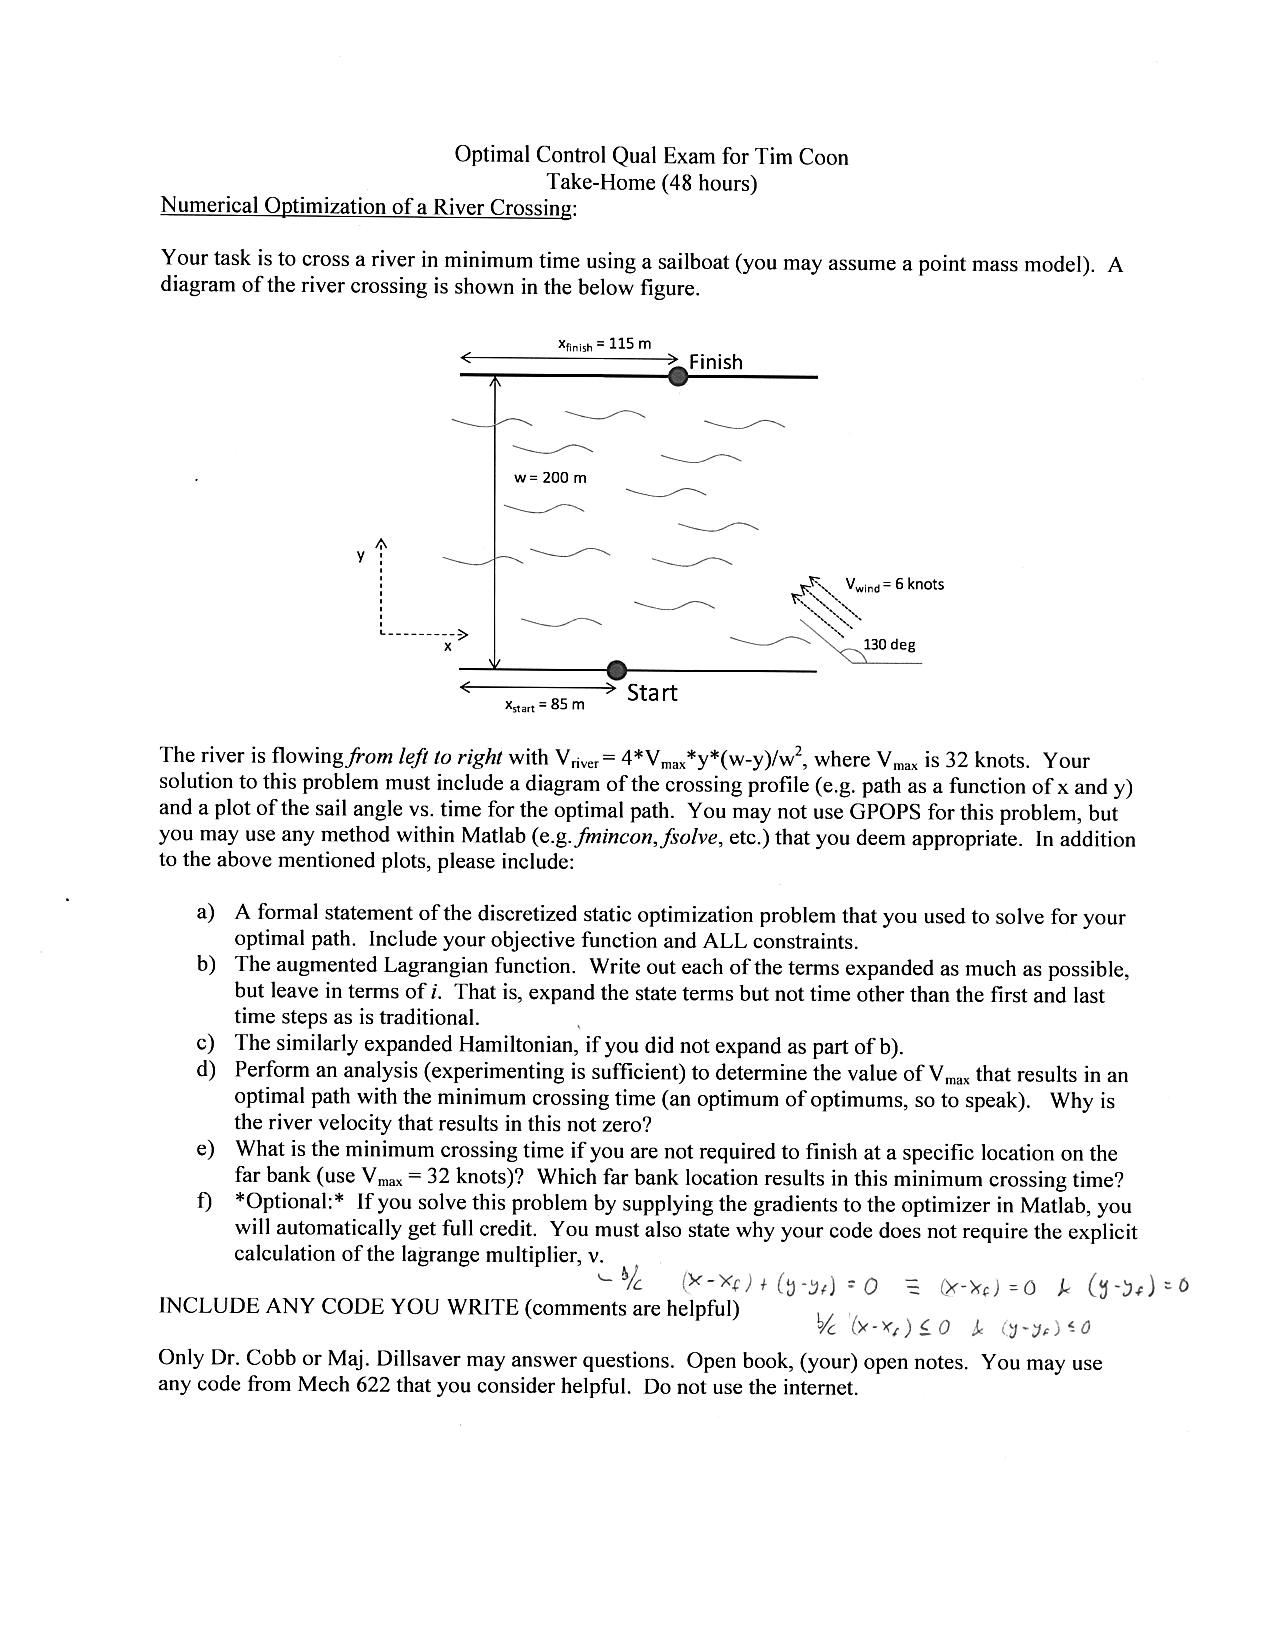
\includegraphics[width=1.0\textwidth]{Q2 MECH622 Problem Statement.pdf}
	\caption{caption}
	\label{fig:Q2 MECH622 Problem Statement}
\end{figure}
\begin{document}
% 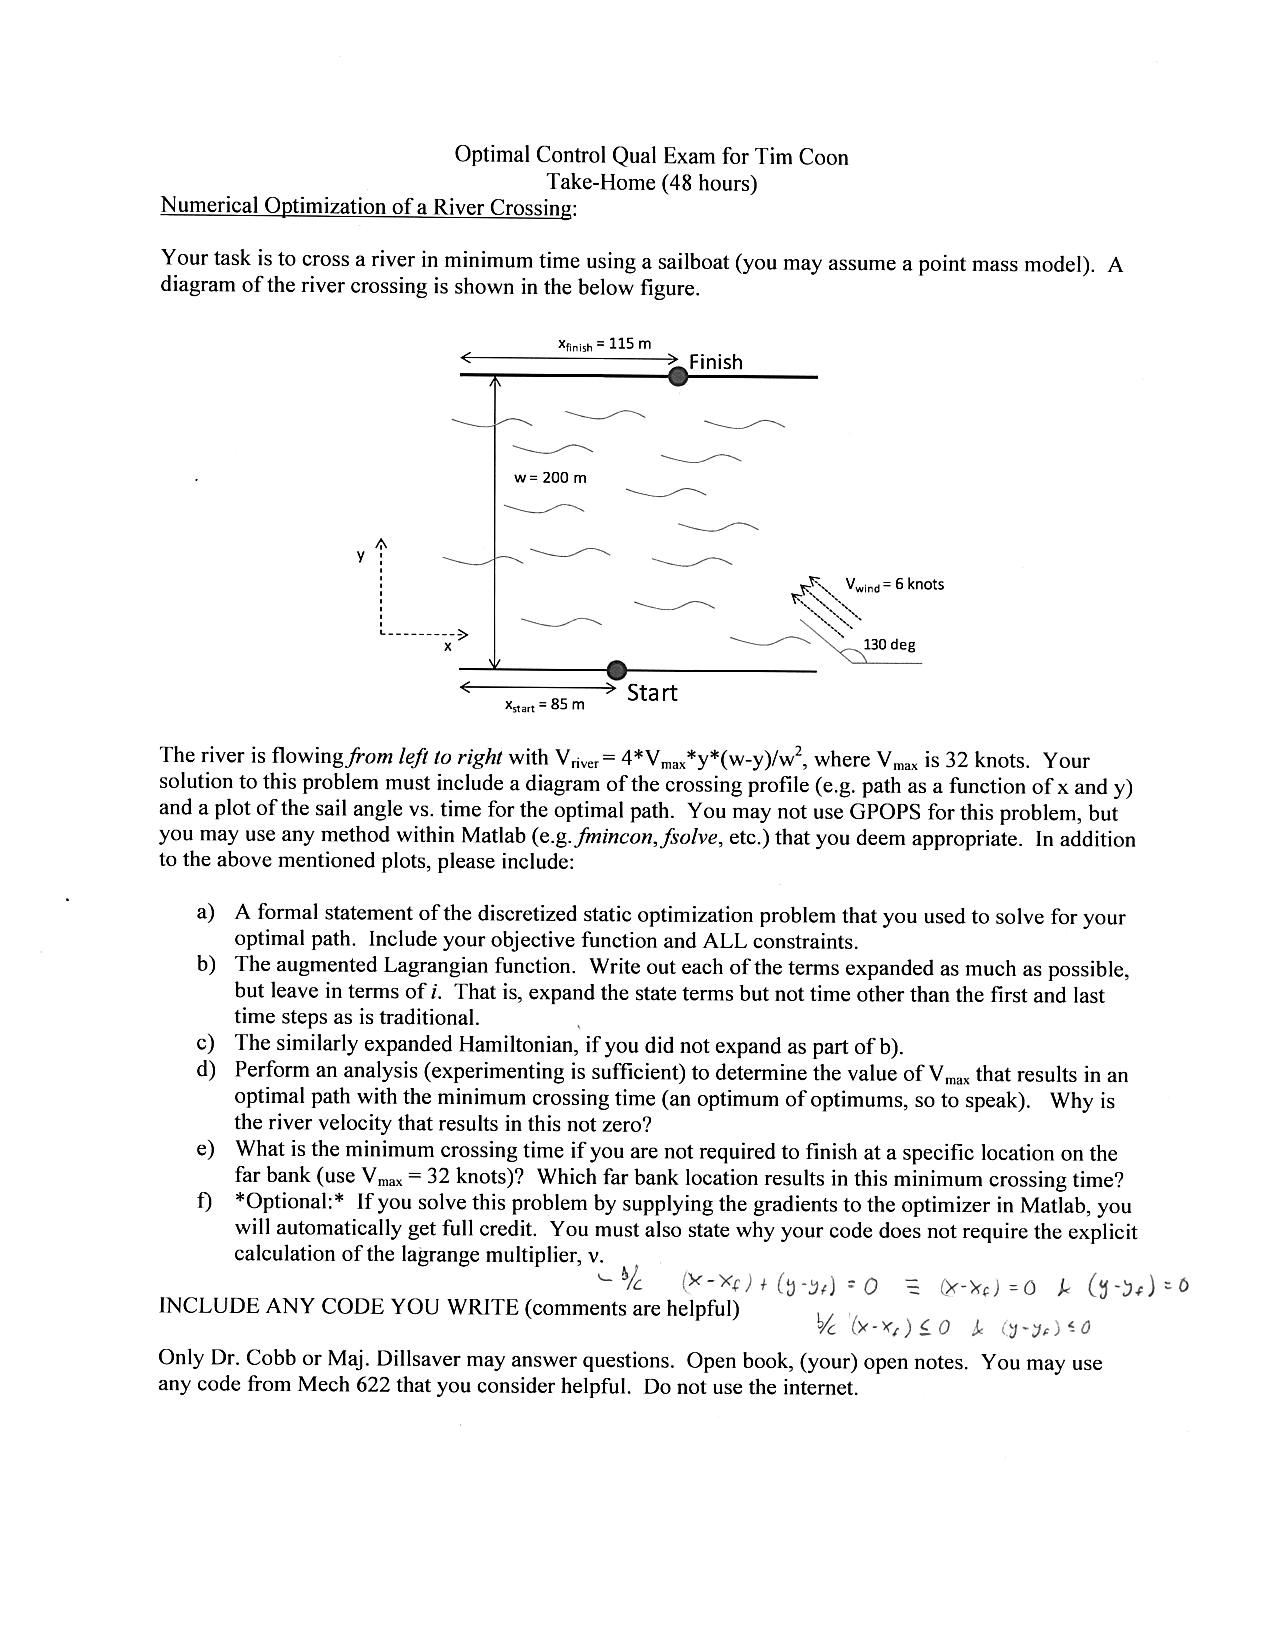
\includepdf[pages={1}]{Q2 MECH622 Problem Statement.pdf}




\AddToShipoutPicture{\BackgroundStructure} % Set the background of each page to that specified above in the header information section

%----------------------------------------------------------------------------------------
%	DOCUMENT CONTENT
%----------------------------------------------------------------------------------------

\subsection*{Problem \#1}

For the differential equation

\begin{align}
	\label{DE}
	\ddot{x}+x = \epsilon x^2, && x(0)=a, && \dot{x}(0), && 0<\epsilon \ll 1 \\
\end{align}

To understand this problem better, find the fixed points and analyze the linear stability of these fixed points. First, put the equation into state-space (or phase-space or first-order) representation.
\begin{align*}
	z_1 &= x, \\ z_2 &= \dot{x} \\
\end{align*}
We have, now, a system of first-order equations: 
\begin{align*}
	\dot{z_1} &= z_2 \\
	\dot{z_2} &= \epsilon z_1^2 - z_1 \\
\end{align*}

To find the stationary (fixed, equilibrium, singular, etc.) points, we set the derivatives equal to zero. This makes sense, intuitively. In reality, the condition must also be that the double derivatives are also equal to zero and this is addressed in some texts. I assume this issue extends to higher-order derivatives for special analysis purposes of irregular systems. For this system, the stationary points are $(0,0)$ and $(0,frac{1}{\epsilon})$.

To perform linear stability analysis, first calculate the Jacobian Matrix.

\begin{align*}
	J &= 
	\begin{bmatrix}
	\dfrac{\partial f_1}{\partial z_1} & \dfrac{\partial f_1}{\partial z_2} \\ \\
	\dfrac{\partial f_2}{\partial z_1} & \dfrac{\partial f_2}{\partial z_2} \\
	\end{bmatrix} \\
	\\
	&= 
	\begin{bmatrix}
	0 & 1 \\ 	\\ 
	(2\epsilon z_1-1) & 0 \\
	\end{bmatrix} \\
\end{align*}

Now, evaluate the Jacobian at each stationary point and find the eigenvalues. The eigenvalues indicate the action of the exponentials of the solutions. What is the Jacobian system? The solution to the Jacobian system describes the behavior of the states (Reference Baker's stability notes (9.7)). 

\begin{align*}
	J(0,0) &= \begin{bmatrix} 0 & 1 \\ -1 & 0 \end{bmatrix} & \lambda_1 &= \pm i \\
	J(\frac{1}{\epsilon},0) &= \begin{bmatrix} 0 & 1 \\ 1 & 0 \end{bmatrix} & \lambda_1 &= \pm 1 \\
\end{align*}

The stationary point $(0,0)$ has purely imaginary eigenvalues of multiplicity 1, so the point is considered stable (marginally stable). The stationary point $(\frac{1}{\epsilon})$ has one positive and one negative eigenvalue, thus, the exponential growth takes over and the point is unstable.

\subsubsection*{Poincar\`{e} Approximate Solution}

Assume the nonlinear differential equation has a solution of the general form:

\begin{equation*}
	x(t,\epsilon) = \delta_0(\epsilon)x_0(t)+\delta_1(\epsilon)x_1(t)+\delta_2(\epsilon)x_2(t)+\cdots
\end{equation*}

To simplify, we assume a more specific form with $\delta_i(\epsilon)=\epsilon^i$ and the solution becomes:

\begin{equation}
	\label{eq:assumedsol}
	x(t,\epsilon) = x_0(t)+\epsilon x_1(t)+\epsilon^2 x_2(t)+\cdots
\end{equation}

Take derivatives and substitute \eqref{eq:assumedsol} into \eqref{eq:DE} and order with coefficients of powers of epsilon: (note: higher order terms are not evaluated)

\begin{equation}
	(\ddot{x}_0+x_0)+\epsilon(\ddot{x}_1+x_1)+\epsilon^2(\ddot{x}_2+x_2) 
		= \epsilon\left[x_0^2+2\epsilon x_0x_1+ h.o.t \right ]
\end{equation}

By equating coefficients of like-power terms of $\epsilon$, develop differential equations to be solved in sequential order.

\begin{align}
	\mathcal{O}(\epsilon^0): && \ddot{x}_0+x_0 &= 0, & x_0(0) &= a, & \dot{x}_0(0) &= 0 \\ \nonumber
	\\
	&& x_0(t) &= a\cos(t)
\end{align}

\begin{align}
	\mathcal{O}(\epsilon^1): && \ddot{x}_1+x_1 &= x_0^2, & x_1(0) &= 0, & \dot{x}_1(0) &= 0 \\ \nonumber
	&& &= a^2\cos^2(t) \\ \nonumber
	&& &= \frac{a^2}{2}(1+\cos(2t))
\end{align}
Solve using the method of undetermined coefficients (``judicial guessing")
\begin{align}
	homogeneous: && x_{1h}(t) &= a_1\cos(t) + b_1\sin(t) &&&\\
	particular: && x_{1p}(t) &= A_1+B_1\cos(2t) &&& \\
	&& &= \frac{a^2}{2}(1-\frac{1}{3}\cos(2t)) \\
	total: && x_1(t) &= a_1\cos(t) + b_1\sin(t) + \frac{a^2}{2}(1-\frac{1}{3}\cos(2t))
\end{align}
Apply initial conditions to find:

\begin{equation}
	x_1(t) = a^2 \left[ \frac{q}{2}-\frac{1}{3}\cos(t)-\frac{1}{6}\cos(2t)\right]
\end{equation}

Substitute into \eqref{eq:assumedsol} to find:

\begin{equation}
	x(t,\epsilon) = \frac{a^2}{2}\epsilon+(a-\frac{a^2}{3}\epsilon)\cos(t)-\frac{a^2}{6}\epsilon\cos(2t)+\mathcal{O}(\epsilon^2)
\end{equation}

This second-order approximation is a well-behaved periodic solution.


\subsubsection*{a) Apply Linstedt's Method to obtain an approximate solution. State the effect of the nonlinear term on the strained frequency and the development of secular terms.}



\subsubsection*{b) Produce an energy function for this system and use it to sketch the phase plane.}



\subsubsection*{c) Show that the center of oscillation can be approximated by $(x_c,0)$}



%----------------------------------------------------------------------------------------
\newpage


%\input{Problem_2}
%\input{Problem_3}
%\input{Problem_4}


\ClearShipoutPicture
% \includepdf[pages={1}]{../OENG644_HW1_P2.pdf}

%----------------------------------------------------------------------------------------

\end{document}